%---------------
%╔═╗╔═╗╔╦╗╦ ╦╔═╗
%╚═╗║╣  ║ ║ ║╠═╝
%╚═╝╚═╝ ╩ ╚═╝╩  
%---------------

% language setup
\newcommand{\docLanguage}{ngerman}
%\newcommand{\docLanguage}{english}

% DOCUMENT SETUP
\documentclass[12pt, oneside, a4paper, \docLanguage]{report}
\usepackage[left=3cm, 
			right=2.5cm, 
			top=2.5cm, 
			bottom=2.5cm, 
			includehead, 
			includefoot]{geometry}

% line spacing
\usepackage{setspace}
\setstretch{1,25} % 15/12 --> 1.25

% encoding setup
% T1 font encoding for languages that use a latin alphabet
\usepackage[T1]{fontenc} 

% enhanced input encoding handling - utf8 for äÄüÜöÖß...
\usepackage[utf8]{inputenc}

%de­fines Adobe Times Ro­man as de­fault text font
\usepackage{mathptmx}
\usepackage{times} % needed for acronym package

%PDF linking package
\usepackage[hidelinks]{hyperref}


% Language Setup
\usepackage[\docLanguage]{babel}
% after babel - set chapter string
\AtBeginDocument{\renewcommand{\chaptername}{}}

% language specific bibliography style
\usepackage[numbers, square]{natbib}
%\setcitestyle{square,aysep={},yysep={;}}
\usepackage[fixlanguage]{babelbib}
\selectbiblanguage{\docLanguage}
% bliographystyle setup
% babel specific: babplain, babplai3, babalpha, babunsrt, bababbrv, bababbr3
\bibliographystyle{babunsrt}


% enumeration
\usepackage{enumitem}
% tabular extension tabularx
\usepackage{tabularx}

% math packages
\usepackage{amsmath}
\usepackage{nicefrac}
\usepackage{amsthm}
\usepackage{amsbsy}
\usepackage{amssymb}
\usepackage{amsfonts}
%\usepackage{MnSymbol}


%special characters
\usepackage{amssymb}
\usepackage{upgreek,textgreek}

% acronym package
\usepackage[printonlyused, footnote]{acronym}

% breakable text in \seqsplit{}
\usepackage{seqsplit}

% \textmu
\usepackage{textcomp}

% package provides a way to compile sections of a document using the same preamble as the main document
\usepackage{subfiles}

% driver-independent color extension - used by listings,tabularx
\usepackage[usenames,dvipsnames,table,xcdraw]{xcolor}

% -- SYNTAX HIGHLIGHTING --
\usepackage{listings}
%% bash command line Syntax Highlighting
\lstdefinestyle{BASH_CMD}{ 
  columns=fullflexible,            % copy pasteable listings
  language=bash,
  basicstyle=\small\sffamily,
  basicstyle   = \small \ttfamily,
  keywordstyle = [1]\small \ttfamily,
  keywordstyle = [2]\small \ttfamily,
  commentstyle = \small \ttfamily,
  numbers=none,
  captionpos=b, 
  breaklines=true,
  numberstyle=\tiny,
  numbersep=3pt,
  frame=tlrb,
  columns=fullflexible,
  backgroundcolor=\color{white!20},
  linewidth=\linewidth,
  literate=                        % replace in code
     {Ö}{{\"O}}1
     {Ä}{{\"A}}1
     {Ü}{{\"U}}1
     {ß}{{\ss}}2
     {ü}{{\"u}}1
     {ä}{{\"a}}1
     {ö}{{\"o}}1
}
 % adds style BASH_CMD
%% Matlab Syntax Highlighting
\colorlet{keyword}{blue!100!black!80}
\colorlet{STD}{Lavender}
\colorlet{comment}{green!90!black!90}
\definecolor{mygreen}{rgb}{0,0.6,0}
\definecolor{mygray}{rgb}{0.5,0.5,0.5}
\definecolor{mymauve}{rgb}{0.58,0,0.82}


\lstdefinestyle{BASH_SCRIPT}{ 
  language     = bash,
  basicstyle   = \footnotesize \ttfamily,
  keywordstyle = [1]\color{keyword}\bfseries,
  keywordstyle = [2]\color{STD}\bfseries,
  commentstyle = \color{mygreen}\itshape,
  backgroundcolor=\color{white},   % choose the background color; you must add \usepackage{color} 
  columns=fullflexible,            % copy pasteable listings
                                   % or \usepackage{xcolor}
  basicstyle=\footnotesize,        % the size of the fonts that are used for the code
  breakatwhitespace=false,         % sets if automatic breaks should only happen at whitespace
  breaklines=true,                 % sets automatic line breaking
  captionpos=b,                    % sets the caption-position to bottom
  extendedchars=true,              % lets you use non-ASCII characters; for 8-bits encodings only,
                                   % does not work with UTF-8
  frame=single,                    % adds a frame around the code
  keepspaces=true,                 % keeps spaces in text, useful for keeping indentation of code
                                   % (possibly needs columns=flexible)
  numbers=left,                    % where to put the line-numbers; possible values are 
                                   % (none, left, right)
  numbersep=5pt,                   % how far the line-numbers are from the code
  numberstyle=\tiny\color{mygray}, % the style that is used for the line-numbers
  rulecolor=\color{black},         % if not set, the frame-color may be changed on line-breaks
                                   % within not-black text (e.g. comments (green here))
  showspaces=false,                % show spaces everywhere adding particular underscores; it
  	                               % overrides 'showstringspaces'
  showstringspaces=false,          % underline spaces within strings only
  showtabs=false,                  % show tabs within strings adding particular underscores
  stepnumber=1,                    % the step between two line-numbers. If it's 1, each line 
                                   % will be numbered
  stringstyle=\color{mymauve},     % string literal style
  tabsize=2,                       % sets default tabsize to 2 spaces
  title=\lstname,                  % set title name
  literate=                        % replace in code
     {Ö}{{\"O}}1 
     {Ä}{{\"A}}1 
     {Ü}{{\"U}}1 
     {ß}{{\ss}}2 
     {ü}{{\"u}}1 
     {ä}{{\"a}}1 
     {ö}{{\"o}}1 
     {â}{{\^{a}}}1 
     {Â}{{\^{A}}}1 
     {ç}{{\c{c}}}1 
     {Ç}{{\c{C}}}1 
     {ğ}{{\u{g}}}1 
     {Ğ}{{\u{G}}}1 
     {ı}{{\i}}1 
     {İ}{{\.{I}}}1 
     {ş}{{\c{s}}}1 
     {Ş}{{\c{S}}}1 
} % adds style BASH_SCRIPT
% Matlab Syntax Highlighting
\colorlet{keyword}{blue!100!black!80}
\colorlet{STD}{red}
\colorlet{comment}{green!90!black!90}
\definecolor{mygreen}{rgb}{0,0.6,0}
\definecolor{mygray}{rgb}{0.5,0.5,0.5}
\definecolor{mymauve}{rgb}{0.58,0,0.82}


\lstdefinestyle{LATEX}{ 
  language     = [LaTeX]{TeX},
  basicstyle   = \footnotesize \ttfamily,
  keywordstyle = [1]\color{keyword}\bfseries,
  keywordstyle = [2]\color{comment}\bfseries,
  commentstyle = \color{mygray}\itshape,
  %backgroundcolor=\color{white},   % choose the background color; you must add \usepackage{color} 
                                   % or \usepackage{xcolor}
  basicstyle=\footnotesize,        		   % the size of the fonts that are used for the code
  breakatwhitespace=false,         % sets if automatic breaks should only happen at whitespace
  columns=fullflexible,            % copy pasteable listings
  breaklines=true,                 % sets automatic line breaking
  captionpos=c,                    % sets the caption-position to bottom
  extendedchars=true,              % lets you use non-ASCII characters; for 8-bits encodings only,
                                   % does not work with UTF-8
  frame=single,                    % adds a frame around the code
  keepspaces=true,                 % keeps spaces in text, useful for keeping indentation of code
                                   % (possibly needs columns=flexible)
  numbers=left,                    % where to put the line-numbers; possible values are 
                                   % (none, left, right)
  numbersep=4pt,                   % how far the line-numbers are from the code
  numberstyle=\tiny\color{mygray}, % the style that is used for the line-numbers
  rulecolor=\color{black},         % if not set, the frame-color may be changed on line-breaks
                                   % within not-black text (e.g. comments (green here))
  showspaces=false,                % show spaces everywhere adding particular underscores; it
  	                               % overrides 'showstringspaces'
  showstringspaces=false,          % underline spaces within strings only
  showtabs=false,                  % show tabs within strings adding particular underscores
  stepnumber=1,                    % the step between two line-numbers. If it's 1, each line 
                                   % will be numbered
  stringstyle=\color{mymauve},     % string literal style
  tabsize=2,                       % sets default tabsize to 2 spaces
  title=\lstname,                  % set title name
  literate=                        % replace in code
     {Ö}{{\"O}}1 
     {Ä}{{\"A}}1 
     {Ü}{{\"U}}1 
     {ß}{{\ss}}2 
     {ü}{{\"u}}1 
     {ä}{{\"a}}1 
     {ö}{{\"o}}1 
     {â}{{\^{a}}}1 
     {Â}{{\^{A}}}1 
     {ç}{{\c{c}}}1 
     {Ç}{{\c{C}}}1 
     {ğ}{{\u{g}}}1 
     {Ğ}{{\u{G}}}1 
     {ı}{{\i}}1 
     {İ}{{\.{I}}}1 
     {ş}{{\c{s}}}1 
     {Ş}{{\c{S}}}1 
} % adds style LATEX
%% Matlab Syntax Highlighting
\colorlet{keyword}{blue!100!black!80}
\colorlet{STD}{Lavender}
\colorlet{comment}{green!90!black!90}
\definecolor{mygreen}{rgb}{0,0.6,0}
\definecolor{mygray}{rgb}{0.5,0.5,0.5}
\definecolor{mymauve}{rgb}{0.58,0,0.82}


\lstdefinestyle{MATLAB}{ 
  language     = Matlab,
  basicstyle   = \footnotesize \ttfamily,
  keywordstyle = [1]\color{keyword}\bfseries,
  keywordstyle = [2]\color{STD}\bfseries,
  commentstyle = \color{mygreen}\itshape,
  backgroundcolor=\color{white},   % choose the background color; you must add \usepackage{color} 
                                   % or \usepackage{xcolor}
  basicstyle=\footnotesize,        % the size of the fonts that are used for the code
  breakatwhitespace=false,         % sets if automatic breaks should only happen at whitespace
  columns=fullflexible,            % copy pasteable listings
  breaklines=false,                % sets automatic line breaking
  captionpos=c,                    % sets the caption-position to bottom
  extendedchars=true,              % lets you use non-ASCII characters; for 8-bits encodings only,
                                   % does not work with UTF-8
  frame=single,                    % adds a frame around the code
  keepspaces=true,                 % keeps spaces in text, useful for keeping indentation of code
                                   % (possibly needs columns=flexible)
  numbers=left,                    % where to put the line-numbers; possible values are 
                                   % (none, left, right)
  numbersep=5pt,                   % how far the line-numbers are from the code
  numberstyle=\tiny\color{mygray}, % the style that is used for the line-numbers
  rulecolor=\color{black},         % if not set, the frame-color may be changed on line-breaks
                                   % within not-black text (e.g. comments (green here))
  showspaces=false,                % show spaces everywhere adding particular underscores; it
  	                               % overrides 'showstringspaces'
  showstringspaces=false,          % underline spaces within strings only
  showtabs=false,                  % show tabs within strings adding particular underscores
  stepnumber=1,                    % the step between two line-numbers. If it's 1, each line 
                                   % will be numbered
  stringstyle=\color{mymauve},     % string literal style
  tabsize=2,                       % sets default tabsize to 2 spaces
  title=\lstname,                  % set title name
  literate=                        % replace in code
     {Ö}{{\"O}}1 
     {Ä}{{\"A}}1 
     {Ü}{{\"U}}1 
     {ß}{{\ss}}2 
     {ü}{{\"u}}1 
     {ä}{{\"a}}1 
     {ö}{{\"o}}1 
     {â}{{\^{a}}}1 
     {Â}{{\^{A}}}1 
     {ç}{{\c{c}}}1 
     {Ç}{{\c{C}}}1 
     {ğ}{{\u{g}}}1 
     {Ğ}{{\u{G}}}1 
     {ı}{{\i}}1 
     {İ}{{\.{I}}}1 
     {ş}{{\c{s}}}1 
     {Ş}{{\c{S}}}1 
} % adds style MATLAB
% Matlab Syntax Highlighting
\colorlet{keyword}{blue!100!black!80}
\colorlet{STD}{Lavender}
\colorlet{comment}{green!90!black!90}
\definecolor{mygreen}{rgb}{0,0.6,0}
\definecolor{mygray}{rgb}{0.5,0.5,0.5}
\definecolor{mymauve}{rgb}{0.58,0,0.82}


\lstdefinestyle{PYTHON}{ 
  language     = Python,
  basicstyle   = \footnotesize \ttfamily,
  keywordstyle = [1]\color{keyword}\bfseries,
  keywordstyle = [2]\color{STD}\bfseries,
  commentstyle = \color{mygreen}\itshape,
  backgroundcolor=\color{white},   % choose the background color; you must add \usepackage{color} 
                                   % or \usepackage{xcolor}
  basicstyle=\footnotesize,        % the size of the fonts that are used for the code
  columns=fullflexible,            % copy pasteable listings
  breakatwhitespace=false,         % sets if automatic breaks should only happen at whitespace
  breaklines=false,                % sets automatic line breaking
  captionpos=c,                    % sets the caption-position to bottom
  extendedchars=true,              % lets you use non-ASCII characters; for 8-bits encodings only,
                                   % does not work with UTF-8
  frame=single,                    % adds a frame around the code
  keepspaces=true,                 % keeps spaces in text, useful for keeping indentation of code
                                   % (possibly needs columns=flexible)
  numbers=left,                    % where to put the line-numbers; possible values are 
                                   % (none, left, right)
  numbersep=5pt,                   % how far the line-numbers are from the code
  numberstyle=\tiny\color{mygray}, % the style that is used for the line-numbers
  rulecolor=\color{black},         % if not set, the frame-color may be changed on line-breaks
                                   % within not-black text (e.g. comments (green here))
  showspaces=false,                % show spaces everywhere adding particular underscores; it
  	                               % overrides 'showstringspaces'
  showstringspaces=false,          % underline spaces within strings only
  showtabs=false,                  % show tabs within strings adding particular underscores
  stepnumber=1,                    % the step between two line-numbers. If it's 1, each line 
                                   % will be numbered
  stringstyle=\color{mymauve},     % string literal style
  tabsize=2,                       % sets default tabsize to 2 spaces
  title=\lstname,                  % set title name
  literate=                        % replace in code
     {Ö}{{\"O}}1 
     {Ä}{{\"A}}1 
     {Ü}{{\"U}}1 
     {ß}{{\ss}}2 
     {ü}{{\"u}}1 
     {ä}{{\"a}}1 
     {ö}{{\"o}}1 
     {â}{{\^{a}}}1 
     {Â}{{\^{A}}}1 
     {ç}{{\c{c}}}1 
     {Ç}{{\c{C}}}1 
     {ğ}{{\u{g}}}1 
     {Ğ}{{\u{G}}}1 
     {ı}{{\i}}1 
     {İ}{{\.{I}}}1 
     {ş}{{\c{s}}}1 
     {Ş}{{\c{S}}}1 
} % adds style PYTHON
%% Matlab Syntax Highlighting
\colorlet{keyword}{blue!100!black!80}
\colorlet{STD}{Lavender}
\colorlet{comment}{green!90!black!90}
\definecolor{mygreen}{rgb}{0,0.6,0}
\definecolor{mygray}{rgb}{0.5,0.5,0.5}
\definecolor{mymauve}{rgb}{0.58,0,0.82}


\lstdefinestyle{CPP}{ 
  language     = C++,
  basicstyle   = \footnotesize \ttfamily,
  keywordstyle = [1]\color{keyword}\bfseries,
  keywordstyle = [2]\color{STD}\bfseries,
  commentstyle = \color{mygreen}\itshape,
  backgroundcolor=\color{white},   % choose the background color; you must add \usepackage{color} 
                                   % or \usepackage{xcolor}
  columns=fullflexible,            % copy pasteable listings
  basicstyle=\footnotesize,        % the size of the fonts that are used for the code
  breakatwhitespace=false,         % sets if automatic breaks should only happen at whitespace
  breaklines=false,                % sets automatic line breaking
  captionpos=c,                    % sets the caption-position to bottom
  extendedchars=true,              % lets you use non-ASCII characters; for 8-bits encodings only,
                                   % does not work with UTF-8
  frame=single,                    % adds a frame around the code
  keepspaces=true,                 % keeps spaces in text, useful for keeping indentation of code
                                   % (possibly needs columns=flexible)
  numbers=left,                    % where to put the line-numbers; possible values are 
                                   % (none, left, right)
  numbersep=5pt,                   % how far the line-numbers are from the code
  numberstyle=\tiny\color{mygray}, % the style that is used for the line-numbers
  rulecolor=\color{black},         % if not set, the frame-color may be changed on line-breaks
                                   % within not-black text (e.g. comments (green here))
  showspaces=false,                % show spaces everywhere adding particular underscores; it
  	                               % overrides 'showstringspaces'
  showstringspaces=false,          % underline spaces within strings only
  showtabs=false,                  % show tabs within strings adding particular underscores
  stepnumber=1,                    % the step between two line-numbers. If it's 1, each line 
                                   % will be numbered
  stringstyle=\color{mymauve},     % string literal style
  tabsize=2,                       % sets default tabsize to 2 spaces
  title=\lstname,                  % set title name
  literate=                        % replace in code
     {Ö}{{\"O}}1 
     {Ä}{{\"A}}1 
     {Ü}{{\"U}}1 
     {ß}{{\ss}}2 
     {ü}{{\"u}}1 
     {ä}{{\"a}}1 
     {ö}{{\"o}}1 
     {â}{{\^{a}}}1 
     {Â}{{\^{A}}}1 
     {ç}{{\c{c}}}1 
     {Ç}{{\c{C}}}1 
     {ğ}{{\u{g}}}1 
     {Ğ}{{\u{G}}}1 
     {ı}{{\i}}1 
     {İ}{{\.{I}}}1 
     {ş}{{\c{s}}}1 
     {Ş}{{\c{S}}}1 
} % adds style CPP
%% Matlab Syntax Highlighting
\colorlet{keyword}{blue!100!black!80}
\colorlet{STD}{Lavender}
\colorlet{comment}{green!90!black!90}
\definecolor{mygreen}{rgb}{0,0.6,0}
\definecolor{mygray}{rgb}{0.5,0.5,0.5}
\definecolor{mymauve}{rgb}{0.58,0,0.82}


\lstdefinestyle{C}{ 
  language     = C,
  basicstyle   = \footnotesize \ttfamily,
  keywordstyle = [1]\color{keyword}\bfseries,
  keywordstyle = [2]\color{STD}\bfseries,
  commentstyle = \color{mygreen}\itshape,
  backgroundcolor=\color{white},   % choose the background color; you must add \usepackage{color} 
  columns=fullflexible,            % copy pasteable listings
                                   % or \usepackage{xcolor}
  basicstyle=\footnotesize,        % the size of the fonts that are used for the code
  breakatwhitespace=false,         % sets if automatic breaks should only happen at whitespace
  breaklines=false,                % sets automatic line breaking
  captionpos=c,                    % sets the caption-position to bottom
  extendedchars=true,              % lets you use non-ASCII characters; for 8-bits encodings only,
                                   % does not work with UTF-8
  frame=single,                    % adds a frame around the code
  keepspaces=true,                 % keeps spaces in text, useful for keeping indentation of code
                                   % (possibly needs columns=flexible)
  numbers=left,                    % where to put the line-numbers; possible values are 
                                   % (none, left, right)
  numbersep=5pt,                   % how far the line-numbers are from the code
  numberstyle=\tiny\color{mygray}, % the style that is used for the line-numbers
  rulecolor=\color{black},         % if not set, the frame-color may be changed on line-breaks
                                   % within not-black text (e.g. comments (green here))
  showspaces=false,                % show spaces everywhere adding particular underscores; it
  	                               % overrides 'showstringspaces'
  showstringspaces=false,          % underline spaces within strings only
  showtabs=false,                  % show tabs within strings adding particular underscores
  stepnumber=1,                    % the step between two line-numbers. If it's 1, each line 
                                   % will be numbered
  stringstyle=\color{mymauve},     % string literal style
  tabsize=2,                       % sets default tabsize to 2 spaces
  title=\lstname,                  % set title name
  literate=                        % replace in code
     {Ö}{{\"O}}1 
     {Ä}{{\"A}}1 
     {Ü}{{\"U}}1 
     {ß}{{\ss}}2 
     {ü}{{\"u}}1 
     {ä}{{\"a}}1 
     {ö}{{\"o}}1 
     {â}{{\^{a}}}1 
     {Â}{{\^{A}}}1 
     {ç}{{\c{c}}}1 
     {Ç}{{\c{C}}}1 
     {ğ}{{\u{g}}}1 
     {Ğ}{{\u{G}}}1 
     {ı}{{\i}}1 
     {İ}{{\.{I}}}1 
     {ş}{{\c{s}}}1 
     {Ş}{{\c{S}}}1 
} % adds style C
%% JSON Syntax Highlighting
\colorlet{keyword}{blue!100!black!80}
\colorlet{STD}{Lavender}
\colorlet{comment}{green!90!black!90}
\definecolor{mygreen}{rgb}{0,0.6,0}
\definecolor{mygray}{rgb}{0.5,0.5,0.5}
\definecolor{mymauve}{rgb}{0.58,0,0.82}

\newcommand\JSONnumbervaluestyle{\color{blue}}
\newcommand\JSONstringvaluestyle{\color{red}}

\newif\ifcolonfoundonthisline

\makeatletter

\lstdefinelanguage{json}
{
  showstringspaces    = false,
  keywords            = {false,true},
  alsoletter          = 0123456789.,
  morestring          = [s]{"}{"},
  morestring          = [s]{'}{'},
  stringstyle         = \ifcolonfoundonthisline\JSONstringvaluestyle\fi,
  MoreSelectCharTable =%
    \lst@DefSaveDef{`:}\colon@json{\processColon@json},
  basicstyle          = \ttfamily,
  keywordstyle        = \ttfamily\bfseries,
}

% flip the switch if a colon is found in Pmode
\newcommand\processColon@json{
  \colon@json%
  \ifnum\lst@mode=\lst@Pmode%
    \global\colonfoundonthislinetrue%
  \fi
}

\lst@AddToHook{Output}{%
  \ifcolonfoundonthisline%
    \ifnum\lst@mode=\lst@Pmode%
      \def\lst@thestyle{\JSONnumbervaluestyle}%
    \fi
  \fi
  %override by keyword style if a keyword is detected!
  \lsthk@DetectKeywords% 
}

% reset the switch at the end of line
\lst@AddToHook{EOL}%
  {\global\colonfoundonthislinefalse}

\makeatother



\lstdefinestyle{JSON}{ 
  language     = json,
  basicstyle   = \footnotesize \ttfamily,
  keywordstyle = [1]\color{keyword}\bfseries,
  keywordstyle = [2]\color{STD}\bfseries,
  commentstyle = \color{mygreen}\itshape,
  backgroundcolor=\color{white},   % choose the background color; you must add \usepackage{color} 
                                   % or \usepackage{xcolor}
  basicstyle=\footnotesize,        % the size of the fonts that are used for the code
  columns=fullflexible,            % copy pasteable listings
  breakatwhitespace=false,         % sets if automatic breaks should only happen at whitespace
  breaklines=false,                % sets automatic line breaking
  captionpos=c,                    % sets the caption-position to bottom
  extendedchars=true,              % lets you use non-ASCII characters; for 8-bits encodings only,
                                   % does not work with UTF-8
  frame=single,                    % adds a frame around the code
  keepspaces=true,                 % keeps spaces in text, useful for keeping indentation of code
                                   % (possibly needs columns=flexible)
  numbers=left,                    % where to put the line-numbers; possible values are 
                                   % (none, left, right)
  numbersep=5pt,                   % how far the line-numbers are from the code
  numberstyle=\tiny\color{mygray}, % the style that is used for the line-numbers
  rulecolor=\color{black},         % if not set, the frame-color may be changed on line-breaks
                                   % within not-black text (e.g. comments (green here))
  showspaces=false,                % show spaces everywhere adding particular underscores; it
  	                               % overrides 'showstringspaces'
  showstringspaces=false,          % underline spaces within strings only
  showtabs=false,                  % show tabs within strings adding particular underscores
  stepnumber=1,                    % the step between two line-numbers. If it's 1, each line 
                                   % will be numbered
  stringstyle=\color{mymauve},     % string literal style
  tabsize=2,                       % sets default tabsize to 2 spaces
  title=\lstname,                  % set title name
  literate=                        % replace in code
     {Ö}{{\"O}}1
     {Ä}{{\"A}}1
     {Ü}{{\"U}}1
     {ß}{{\ss}}2
     {ü}{{\"u}}1
     {ä}{{\"a}}1
     {ö}{{\"o}}1
} % adds style JSON

% HEADLINE CFG
\usepackage{fancyhdr} % Headers and footers
\usepackage{lastpage}
\usepackage{ifthen}
\setlength{\headheight}{1.5cm}
%\pagestyle{fancy} % All pages have headers and footers
% override plain page style for \part, \chapter or 
% \maketitle, which implicit specifies plain page style
\fancypagestyle{plain} 
{
	\fancyhead[L]{}
	\fancyhead[C]{}
	\fancyhead[R]{}
	\fancyfoot[L]{}
	\fancyfoot[C]{\thepage}
	\fancyfoot[R]{}
}
% set list pagestyle
\fancypagestyle{preface} 
{
	\fancyhead[L]{}
	\fancyhead[C]{}
	\fancyhead[R]{}
	\fancyfoot[L]{}
	\fancyfoot[C]{\thepage}
	\fancyfoot[R]{}
}
% set default pagestyle
\fancypagestyle{default} 
{
	\fancyhead{} % Blank out the default header
	\fancyfoot{} % Blank out the default footer
	\fancyhead[L]{}
	\fancyhead[C]{}
	\fancyhead[R]{}
	\fancyfoot[L]{}
	\fancyfoot[C]{\thepage}
	\fancyfoot[R]{}
}
%\fancypagestyle{default} 
{
\fancyhead[L]{\ifthenelse{\isodd{\value{page}}}{\arabic{chapter} \rightmark}{}}
\fancyhead[R]{\thepage}
}

\renewcommand{\chaptermark}[1]{\markright{#1}{}}
\renewcommand{\sectionmark}[1]{\markright{#1}{}}
\renewcommand{\headrulewidth}{0pt}
\renewcommand{\footrulewidth}{0pt}

% PICTURE CFG 
\usepackage{verbatim}
\usepackage{graphicx}
\usepackage{epstopdf}
\usepackage{caption}
\usepackage[list=true,listformat=simple]{subcaption}
% floating prevention packages
\usepackage{float}    % used with [H] positioning parameter
\usepackage{placeins} % \FloatBarrier 
% tikz packages
\usepackage{tikz}
\usepackage{standalone}
\usepackage{pgfplots}


% include only specified tex files - uncommend here
\includeonly{preface/cover,
             preface/abstract,
             preface/tableofcontents,
             preface/listoffigures,
             preface/listoftables,
             preface/lstlistoflistings,
             appendix/bibliography}

%-------------------
%╔═╗╔╦╗╦═╗╦╔╗╔╔═╗╔═╗
%╚═╗ ║ ╠╦╝║║║║║ ╦╚═╗
%╚═╝ ╩ ╩╚═╩╝╚╝╚═╝╚═╝
%-------------------
\newcommand{\strLecture}{Signale, Systeme und Sensoren}
\newcommand{\strDate}{\today}
\newcommand{\strAuthorA}{Daniel Wollmann}
\newcommand{\strAuthorB}{Vlad Bratulescu}
%\newcommand{\strAuthorC}{C. Author}
\newcommand{\strAuthorAEmail}{da161wol@htwg-konstanz.de}
\newcommand{\strAuthorBEmail}{vl161bra@htwg-konstanz.de}
%\newcommand{\strAuthorCEmail}{cauthor@htwg-konstanz.de}
% Versuchsbeschreibung 
\newcommand{\strTopic}{Kalibrierung und Einsatz eines Infrarot-Entfernungsmessers}
\newcommand{\strAbstract}{In diesem Versuch werden die in der Vorlesung behandelten Techniken zur Kalibrierung, Fehleranalyse und Fehlerrechnung auf den Fall eines Entfernungsmessers angewandt. Zur Berechnung der Distanz wird ein Sensor verwendet, der nach dem Triangulationsprinzip arbeitet. 

Dabei wird ein Lichtstrahl ausgesendet, welcher vom Objekt reflektiert und zu einem optischen Positionssensor gelenkt wird. Die Leitfähigkeit dieses OPS ist abhängig davon, an welcher Stelle der Lichtstrahl einfällt. Sie wird mit einem Signalprozessor in eine Spannung umgewandelt, die am Ausgang des Sensors ausgegeben wird. 

Die Ausgangsspannung ist anti-proportional zur steigenden Entfernung. Laut Datenblatt liegt der Messbereich des Sensors zwischen 10 cm und 80 cm.}
% hyperref customization
\hypersetup{
	pdftitle     = {\strTopic}, % title
	pdfsubject   = {\strLecture}, % subject of the document
	pdfauthor    = {\strAuthorA, \strAuthorB}, % author
	pdfkeywords  = {}, % list of keywords
	pdfcreator   = {}, % creator of the document
	pdfproducer  = {}, % producer of the document
	colorlinks   = false, % false: boxed links; true: colored links
	linkcolor    = red, % color of internal links (change box color with linkbordercolor)
    citecolor    = green, % color of links to bibliography
    filecolor    = magenta, % color of file links
    urlcolor     = cyan, % color of external links
	%bookmarks    = true, % show bookmarks bar?
	unicode	     = true, % non-Latin characters in Acrobat’s bookmarks
	pdftoolbar   = true, % show Acrobat’s toolbar?
	pdfmenubar   = true, % show Acrobat’s menu?
    pdffitwindow = false, % window fit to page when opened
	pdfnewwindow = true % links in new PDF window
}

%-----------------------------------------
% ╔╗ ╔═╗╔═╗╦╔╗╔  ╔╦╗╔═╗╔═╗╦ ╦╔╦╗╔═╗╔╗╔╔╦╗ 
% ╠╩╗║╣ ║ ╦║║║║   ║║║ ║║  ║ ║║║║║╣ ║║║ ║  
% ╚═╝╚═╝╚═╝╩╝╚╝  ═╩╝╚═╝╚═╝╚═╝╩ ╩╚═╝╝╚╝ ╩  
%-----------------------------------------

\begin{document}
\pagenumbering{Roman} 

\setcounter{section}{0}

\begin{titlepage}

\vspace*{-3.5cm}

\begin{flushleft}
\hspace*{-1cm} 
\includegraphics[width=15.7cm]{preface/htwg-logo}
\end{flushleft}

\vspace{1cm}

\begin{center}
	\large{
		\textbf{\strLecture} \\[2cm]
	}
	\Huge{
		\textbf{\strTopic} \\[2cm]
	}
	\Large{
		\textbf{\strAuthorA, \strAuthorB}} \\[3cm]
		%\textbf{\strAuthorA, \strAuthorB, \strAuthorC}} \\[3cm]
	\large{
		\textbf{} \\[2.3cm]
	}
	
	\large{
		\textbf{Konstanz, \strDate}
	}
\end{center}

\end{titlepage}
\thispagestyle{empty}




\begin{center}
{\Large \textbf{Zusammenfassung (Abstract)}}
\end{center}

\bigskip

\begin{center}
	\begin{tabular}{p{2.8cm}p{5cm}p{5cm}}
		Thema: & \multicolumn{2}{p{10cm}}{\raggedright\strTopic} \\
		 & & \\
		Autoren: & \strAuthorA & \href{mailto:\strAuthorAEmail}{\strAuthorAEmail} \\
		 & \strAuthorB & \href{mailto:\strAuthorBEmail}{\strAuthorBEmail} \\
		 & & \\
		Betreuer: & Prof. Dr. Matthias O. Franz & \href{mailto:mfranz@htwg-konstanz.de}{mfranz@htwg-konstanz.de} \\
		 &  Jürgen Keppler & \href{mailto:juergen.keppler@htwg-konstanz.de}{juergen.keppler@htwg-konstanz.de} \\
		 &  Martin Miller & \href{mailto:martin.miller@htwg-konstanz.de}{martin.miller@htwg-konstanz.de} \\
	\end{tabular}
\end{center}

\bigskip

\noindent
\strAbstract

\thispagestyle{lists}



\clearpage

%
% TABLE OF CONTENTS
%
\pagestyle{preface}
%
% TABLE OF CONTENTS
%
\tableofcontents
\newpage


%
% Abbildungsverzeichnis
%
%
% Abbildungsverzeichnis
%
\phantomsection
\addcontentsline{toc}{chapter}{Abbildungsverzeichnis}
\listoffigures
\thispagestyle{preface}
\newpage
\clearpage

%
% Tabellenverzeichnis
%
%
% Tabellenverzeichnis
%
\phantomsection
\addcontentsline{toc}{chapter}{Tabellenverzeichnis}
\listoftables
\thispagestyle{lists}
\newpage

%
% Listingverzeichnis
%
%
% Listingverzeichnis
%
\phantomsection
\renewcommand\lstlistingname{Listing}
\renewcommand\lstlistlistingname{Listingverzeichnis}
\lstlistoflistings
\addcontentsline{toc}{chapter}{Listingverzeichnis}
\thispagestyle{lists}
\newpage


%--------------------------
% ╔═╗╦ ╦╔═╗╔═╗╔╦╗╔═╗╦═╗╔═╗ 
% ║  ╠═╣╠═╣╠═╝ ║ ║╣ ╠╦╝╚═╗ 
% ╚═╝╩ ╩╩ ╩╩   ╩ ╚═╝╩╚═╚═╝ 
%--------------------------

\pagenumbering{arabic} 
\setcounter{page}{1} 
\pagestyle{default}
%
% CHAPTER Einleitung
%
\chapter{Einleitung}
\label{chap:EINL}
In diesem Versuch wird ein Distanzsensor der Firma Sharp (GP2Y0A21YK0F, siehe Datenblatt in Moodle) kalibriert.

Dabei werden 20 Messungen mit verschiedenen Entfernungen durchgeführt und die Ausgangsspannung aufgezeichnet. 

Mithilfe der Software PicoScope 6 werden die Messwerte auch in digitaler Form als .csv Dateien gespeichert, welche mit einem Python Skript weiter verarbeiten werden können. Dazu gehört die Berechnung des Mittelwerts und der Standardabweichung.

Um die Ausgleichsfunktion zu bestimmen, wird das Verfahren der Linearen Regression angewendet.

Durch die Ausgleichsfunktion kann die Ausgangsspannung in die Distanz umgerechnet werden und die Fläche eines DIN-A4 Blatts anhand der gemessenen Länge und Breite berechnet werden. Um die Genauigkeit dieser Fläche zu bestimmen, wird eine Fehlerrechnung anhand der in der Vorlesung besprochenen Verfahren durchgeführt.
%
% CHAPTER Versuch 1
%
\chapter{Versuch 1}
\label{chap:VERSUCH_1}

\section{Fragestellung, Messprinzip, Aufbau, Messmittel}
\label{chap:VERSUCH_1_FRAGESTELLUNG}
Im Versuch 1 soll Kennlinie des Sensors mithilfe mehrer Messungen an gleichmäßigen Abständen zwischen 10 cm und 70 cm ermittelt werden. Die Messungen sollen sowohl automatisch mittels einer Software, sowie von Hand erfasst werden.

Der Distanzsensor wird mit einer Spannungsquelle von 5 V Gleichspannung versorgt. Des weiteren werden die Anschlüsse für Signalausgang und Ground mit dem Osziloskop verbunden. Das Osziloskop wird per USB-Anschluss mit dem Computer verbunden, um die Messwerte automatisch zu erfassen.

Als Messobjekt wird eine weiße Holzplatte in festgelegten Abständen vor dem Sensor platziert und die Messung durchgeführt. Es werden 20 Messungen mit verschiedenen Distanzen vorgenommen. Die Messungen werden in gleichmäßigen Abständen zwischen 10 und 70 cm durchgeführt. Zur Platzierung der Holzplatte wird ein Meterstab verwendet.

Die Erfassung der Messwerte erfolgen von Hand, sowie auch durch das Computerprogramm PicoScope 6.

Herr Keppler hat den Versuch online über ein WebEx Meeting für uns durchgeführt.
\section{Messwerte}
\label{chap:VERSUCH_1_MESSWERTE}
Tabelle [\ref{fig:VERSUCH_1_MESSWERTE_TABELLE}] zeigt die handschriftlich aufgeschriebenen sowie per Python-Skript berechneten Spannungsmittelwerte der verschiedenen Distanzen. Zusätzlich werden auch die jeweiligen Standardabweichungen berechnet.

Bemerkung: die berechneten Mittelwerte wurden von den bereitgestellten Daten aus Moodle berechnet und stehen nicht in Zusammenhang mit den von Hand aufgeschriebenen Spannungen.
\begin{table}[]
\begin{tabular}{|l|l|l|l|l|}
\hline
\textbf{Nr.} & \textbf{Entfernung {[}cm{]}} & \textbf{Spannung {[}V{]}} & \textbf{Spannung .py Skript {[}V{]}} & \textbf{$\sigma$ .py Skript {[}V{]}} \\ \hline
1            & 70                           & 0,448                     & 0,356                                   & 0,0175                                            \\ \hline
2            & 67                           & 0,514                     & 0,357                                   & 0,0175                                            \\ \hline
3            & 65                           & 0,525                     & 0,396                                   & 0,0176                                            \\ \hline
4            & 62                           & 0,523                     & 0,434                                   & 0,0175                                            \\ \hline
5            & 60                           & 0,565                     & 0,453                                   & 0,0174                                            \\ \hline
6            & 57                           & 0,610                     & 0,473                                   & 0,0173                                            \\ \hline
7            & 55                           & 0,627                     & 0,496                                   & 0,0174                                            \\ \hline
8            & 52                           & 0,610                     & 0,535                                   & 0,0169                                            \\ \hline
9            & 50                           & 0,545                     & 0,575                                   & 0,0170                                            \\ \hline
10           & 47                           & 0,553                     & 0,612                                   & 0,0168                                            \\ \hline
11           & 43                           & 0,608                     & 0,632                                   & 0,0176                                            \\ \hline
12           & 40                           & 0,616                     & 0,671                                   & 0,0174                                            \\ \hline
13           & 37                           & 0,635                     & 0,709                                   & 0,0175                                            \\ \hline
14           & 33                           & 0,671                     & 0,749                                   & 0,0177                                            \\ \hline
15           & 30                           & 0,713                     & 0,807                                   & 0,0173                                            \\ \hline
16           & 27                           & 0,752                     & 0,907                                   & 0,0170                                            \\ \hline
17           & 22                           & 0,866                     & 0,983                                   & 0,0172                                            \\ \hline
18           & 18                           & 0,972                     & 1,078                                   & 0,0172                                            \\ \hline
19           & 14                           & 1,139                     & 1,196                                   & 0,0173                                            \\ \hline
20           & 10                           & 1,353                     & 1,341                                   & 0,0217                                            \\ \hline                           
\end{tabular}
\caption{Messwerte Kalibrierung}
\label{fig:VERSUCH_1_MESSWERTE_TABELLE}
\end{table}
\section{Auswertung}
\label{chap:VERSUCH_1_AUSWERTUNG}
Als nächstes werden die Daten mit Python eingelesen. Mithilfe der Spannungen können dann der Mittelwert und die Standardabweichung zu den einzelnen Dateien berechnet werden. 
Zur Veranschaulichung werden mit einem Python Skript \ref{chap:APPENDIX_SOURCECODE_V1} die Abbildungen \ref{fig:VERSUCH_1_AUSWERTUNG_PLOT} und \ref{fig:VERSUCH_1_AUSWERTUNG_PLOT2} erstellt.
\begin{figure}[H]
	\centering\small
	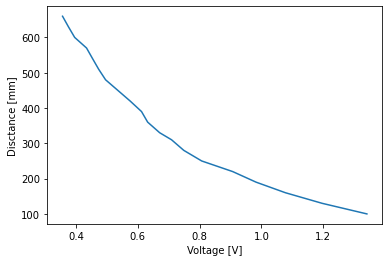
\includegraphics[width=\textwidth]{media/plot_versuch1_spannung_abstand}
	\caption{Spannung und Distanz}
	\label{fig:VERSUCH_1_AUSWERTUNG_PLOT}

	\centering\small
	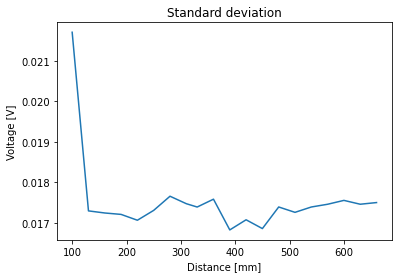
\includegraphics[width=\textwidth]{media/plot_versuch1_abstand_abweichung.png}
	\caption{Standardabweichung und Distanz}
	\label{fig:VERSUCH_1_AUSWERTUNG_PLOT2}
\end{figure}
\section{Interpretation}
\label{chap:VERSUCH_1_INTERPRETATION}
Die Auswertung der Messwerte verdeutlicht die anti-proportional Ausgangsspannung zur Distanz.

Es ist zu erkennen, dass die von Hand aufgeschriebenen Spannungen teilweise sehr ungenau sind, da zum Beispiel die handschriftlichen Messungen 6 bis 10 ein Verhalten zeigen, dass die Anti-Proportionalität nicht widerspiegelt.

Die ermittelten Spannungen des Python Skripts zeigen ein deutlich akkurateres Ergebnis, da 1500 Einzelmessungen zur Berechnung verwendet wurden.
%
% CHAPTER Versuch 2
%
\chapter{Versuch 2}
\label{chap:VERSUCH_2}

\section{Fragestellung, Messprinzip, Aufbau, Messmittel}
\label{chap:VERSUCH_2_FRAGESTELLUNG}
In Versuch 2 war es die Aufgabe alle Distanzen und Mittelwerte der von Hand aufgeschriebenen Spannungen aus der Tabelle zu logarithmieren und den Zusammenhang graphisch darzustellen. Hierbei soll die resultierende Kennlinie die Form einer Geraden haben. 

Anschließend wird mithilfe der linearen Regression die Ausgleichsgerade in Python berechnet. 

Allerdings lässt sich dieses Verfahren nur bei einer linearen Kennlinie anwenden, welcher bei unserem Sensor nicht vorliegt. Um das Verfahren trotzdem nutzen zu können, wurde der im Aufgabenblatt beschriebene Lösungsansatz verwendet.

Für den Versuch werden lediglich die manuell erfassten Daten in der Tabelle [\ref{fig:VERSUCH_1_MESSWERTE_TABELLE}] benötigt und ein Python Skript, das mittels der Formeln und den Daten die Berechnung durchführt.
\newpage
\section{Messwerte}
\label{chap:VERSUCH_2_MESSWERTE}
Tabelle  [\ref{fig:VERSUCH_2_MESSWERTE_TABELLE}]  zeigt die in Python logarithmierten Werte.

\begin{table}[ht!]
\centering
\begin{tabular}{|l|l|l|}
\hline
\textbf{Entfernung {[}cm{]}} & \textbf{log mean} & \textbf{log distance} \\ \hline
70                           & -0,80296              & 6,55108           \\ \hline
67                           & -0,66553              & 6,50728           \\ \hline
65                           & -0,64436              & 6,47697           \\ \hline
62                           & -0,64817              & 6,42972           \\ \hline
60                           & -0,57093              & 6,39693           \\ \hline
57                           & -0,49430              & 6,34564           \\ \hline
55                           & -0,46681              & 6,30992           \\ \hline
52                           & -0,49430              & 6,25383           \\ \hline
50                           & -0,60697              & 6,21461           \\ \hline
47                           & -0,59240              & 6,15273           \\ \hline
43                           & -0,49758              & 6,06379           \\ \hline
40                           & -0,48451              & 5,99146           \\ \hline
37                           & -0,45413              & 5,91350           \\ \hline
33                           & -0,39899              & 5,79909           \\ \hline
30                           & -0,33827              & 5,70378           \\ \hline
27                           & -0,28502              & 5,59842           \\ \hline
22                           & -0,14387              & 5,39363           \\ \hline
18                           & -0,02840              & 5,19296           \\ \hline
14                           & 0,13015               & 4,94164           \\ \hline
10                           & 0,30232               & 4,60517           \\ \hline
\end{tabular}
\caption{Logarithmierte Messwerte}
\label{fig:VERSUCH_2_MESSWERTE_TABELLE}
\end{table}
\newpage
\section{Auswertung}
\label{chap:VERSUCH_2_AUSWERTUNG}

Die manuell erfassten Spannungen und Distanzen werden jeweils mithilfe eines Python Skripts \ref{chap:APPENDIX_SOURCECODE_V2} logarithmiert. Deren Zusammenhang wird dann in Abbildung \ref{fig:VERSUCH_2_MESSWERTE_PLOT2} dargestellt.

Mithilfe der linearen Regression, soll dazu auch die Ausgleichsgerade berechnet werden. Die in der Vorlesung vorgestellte Methode der linearen Regression, funktioniert für den Sharp-Sensor nicht, da er die nichtlineare Kennlinie der Form

\[ y = x^a \]
besitzt. Aus diesem Grund wird auf die obere Gleichung die doppelte Logarithmierung angewendet, sodass sich der folgende Zusammenhang daraus ergibt:

\[ y' = a \cdot x' + b \]
wobei \(x'\) hier die logarithmierte Spannung und \(y'\) der logarithmierte Abstand darstellt. Die Parameter dieser Gerade lassen sich dann durch die lineare Regression schätzen.
\[ a = -1.915981 \]
\[ b = 5,157991 \]
Abbildung \ref{fig:VERSUCH_2_MESSWERTE_PLOT2} stellt diese Ausgleichungsgerade dar.

Die Rückrechnung auf den ursprünglichen Zusammenhang geschieht über die Umkehrung
der doppelten Logarithmierung:
\[ y = exp(a \cdot ln x + b) = e^{5,157991} + x^{-1,915981} \]
wobei \(x\) hier die Spannungsmessung und \(y\) die daraus resultierende Abstandsmessung darstellt.
In Abbildung \ref{fig:VERSUCH_2_MESSWERTE_PLOT3} wird die nichtlineare Kennlinie des Sensors gezeigt.
\begin{figure}[H]
	\centering\small
	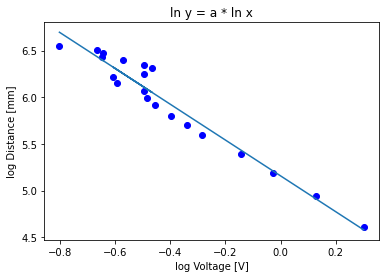
\includegraphics[width=\textwidth]{media/plot_versuch2_logAbstand_logSpannung_regression.png}
	\caption{Lineare Regression}
	\label{fig:VERSUCH_2_MESSWERTE_PLOT2}

	\centering\small
	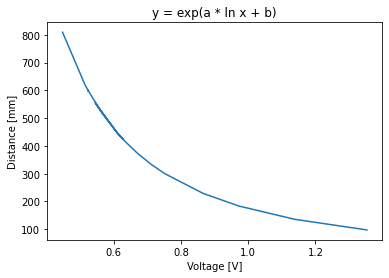
\includegraphics[width=\textwidth]{media/plot_versuch2_spannung_abstand_regression.png}
	\caption{Kennlinie des Sensors}
	\label{fig:VERSUCH_2_MESSWERTE_PLOT3}
\end{figure}
\section{Interpretation}
\label{chap:VERSUCH_2_INTERPRETATION}
In Abbildung \ref{fig:VERSUCH_2_MESSWERTE_PLOT2} kann man im Bereich von 6.25 mm Unstimmigkeiten erkennen. Der Spannungswert steigt in diesem Bereich und fällt dann wieder zurück auf die Kennlinie der Gerade. Da wegen der aktuellen Situation die Messung nicht von uns selber gemacht wurde, können wir die Ursache nicht genau bestimmen. Es ist anzunehmen, dass die Messungen dieser Abstände nicht korrekt durchgeführt wurden.

Abbildung \ref{fig:VERSUCH_2_MESSWERTE_PLOT2} zeigt die Ausgleichsgerade der einzelnen Punkte. Diese scheint minimal beeinflusst von den einzelnen Ausreißern. Die andere Punkte liegen sehr nah an der Geraden.

Zum Schluss wird in Abbildung \ref{fig:VERSUCH_2_MESSWERTE_PLOT3} die nichtlineare Kennlinie des Sensors berechnet. Diese zeigt, dass die Parameter \(a\) und \(b\) trotz des beschriebenen Messfehlers gut geschätzt werden konnten.
% CHAPTER Versuch 3
%
\chapter{Versuch 3}
\label{chap:VERSUCH_3}

\section{Fragestellung, Messprinzip, Aufbau, Messmittel}
\label{chap:VERSUCH_3_FRAGESTELLUNG}
Der dritte Versuch beschäftigt sich mit der Ermittlung des Messfehlers des Abstandssensors. Zu Beginn soll die lange Seite eines DIN-A4 Blattes gemessen werden und die Daten in einer .csv Datei gesichert werden. Zur Ermittlung des Messfehlers muss die Fehlerfortpflanzung durch die Kennlinie $e^b \cdot x^a$ (siehe Abbildung \ref{fig:VERSUCH_2_MESSWERTE_PLOT3}) berechnet werden.

Des Weiteren soll der Vertrauensbereich für eine Sicherheit von 68\% und 95\% berechnet werden. Anschließend kann mithilfe der Fehlerfortpflanzung das Ergebnis der Abstandsmessung in korrekter Form in cm angegeben werden. 

Der Zweite Teil des Versuches beschäftigt sich mit der Breite eines DIN-A4 Blattes und der gleichen Rechenmethode wie im ersten Teil des Versuches. Durch die ermittelte Breite und Länge des DIN-A4 Blattes kann nun der Flächeninhalt berechnet werden. Für die Flächenberechnung wird das Gaußsche Fehlerfortpflanzungsgesetz aus der Vorlesung angewandt. 
\newpage
\section{Messwerte}
\label{chap:VERSUCH_3_MESSWERTE}
In der Tabelle [\ref{fig:VERSUCH_3_MESSWERTE_TABELLE}] sind die handschriftlich notierten Spannungen zu der Länge, wie auch der Breite des gemessenen DIN-A4 Blattes zu sehen.
\begin{table}[H]
\centering
\begin{tabular}{|l|l|}
\hline
\textbf{Entfernung {[}cm{]}} & \textbf{Durchschnittliche Spannung {[}V{]}} \\ \hline
29,7                         & 0,693                                       \\ \hline
21                           & 0,890                                       \\ \hline
\end{tabular}
\caption{Handschriftlich notierte Spannung zur Länge und Breite}
\label{fig:VERSUCH_3_MESSWERTE_TABELLE}
\end{table}

\section{Auswertung}
\label{chap:VERSUCH_3_AUSWERTUNG}
Die Tabelle [\ref{fig:VERSUCH_3_AUSWERTUNG_LAENGE_TABELLE}] zeigt die berechneten Messfehler im Vertrauensbereich von 68\% und 95\% für die lange Seite des DIN-A4 Blattes mit 29,7 cm. 
\begin{table}[H]
\centering
\begin{tabular}{|l|l|l|}
\hline
\textbf{Vertrauensbereich} & \textbf{Spannung von {[}V{]}} & \textbf{Spannung bis {[}V{]}} \\ \hline
68\%                       & 0.675296                      & 0.710704                      \\ \hline
95\%                       & 0.658300                      & 0.727700                      \\ \hline
\end{tabular}
\caption{Messfehler in Gaußverteilung für die Länge}
\label{fig:VERSUCH_3_AUSWERTUNG_LAENGE_TABELLE}
\end{table}

Für die Berechnung des Vertrauensbereichs wurde die Formel $x = \bar x \pm t \cdot \sigma$ verwendet. Wobei t der Korrekturfaktor ist und bei 68\% den Faktor 1 hat und bei 95\% bei 1,96 liegt.

Die Schätzung des Messfehlers wurde ebenfalls mit der selben Methode für die Breite des Blattes durchgeführt. Das Ergebnis für die Breite mit 21 cm sehen wir in Tabelle  [\ref{fig:VERSUCH_3_AUSWERTUNG_BREITE_TABELLE}]

\begin{table}[H]
\centering
\begin{tabular}{|l|l|l|}
\hline
\textbf{Vertrauensbereich} & \textbf{Spannung von {[}V{]}} & \textbf{Spannung bis {[}V{]}} \\ \hline
68\%                       & 0.872955                      & 0.907045                      \\ \hline
95\%                       & 0.856592                      & 0.923408                      \\ \hline
\end{tabular}
\caption{Messfehler in Gaußverteilung für die Breite}
\label{fig:VERSUCH_3_AUSWERTUNG_BREITE_TABELLE}
\end{table}

%In Python wurde die Berechnung wie folgt umgesetzt: \break
%interval68L = [Durchschnittliche Spannung - Standardabweichung, Durchschnittliche Spannung + Standardabweichung] \break
%interval95L = [Durchschnittliche Spannung - 1.96 * Standardabweichung, Durchschnittliche Spannung + 1.96 * Standardabweichung]

Um das Ergebnis in Korrekter Form anzeigen zu können, mittels der Fehlerfortpflanzung, muss zuvor $\Delta x$ für jeweils die Länge und Breite berechnet werden. 

Die Berechnung ergibt sich aus folgender Formel:  $\Delta x = \frac{\sigma}{\sqrt[]{n}}$. Wobei n die Anzahl der Messungen ist. Für das Vertrauensintervall von 95\% muss die Standardabweichung noch mit dem Korrekturfaktor von 1,96 multipliziert werden.

Zusätzlich muss die Funktion $e^b \cdot x^a$ abgeleitet und mit dem errechneten Delta Wert multipliziert werden. Die Ableitung der Funktion sieht wie folgt aus: $a \cdot e^b \cdot x^{a-1}$

Jetzt kann alles eingesetzt werden und die Länge und Breite für die zwei Vertrauensbereiche errechnet werden.

In der nachfolgenden Tabelle [\ref{fig:VERSUCH_3_AUSWERTUNG_ERGEBNISSE_IN_CM_TABELLE}] sind die Ergebnisse veranschaulicht.
\begin{table}[]
\centering
\begin{tabular}{|l|l|l|}
\hline
\textbf{Vertrauensbereich} & \textbf{Errechnete Entfernung {[}cm{]}} & \textbf{Delta +- {[}cm{]}} \\ \hline
68\%                       & 21.729754                               & 0.020588                   \\ \hline
68\%                       & 35.094505                               & 0.044353                   \\ \hline
95\%                       & 21.729754                               & 0.040352                   \\ \hline
95\%                       & 35.094505                               & 0.086933                   \\ \hline
\end{tabular}
\caption{Abstandsmessung mit Fehlerfortpflanzung}
\label{fig:VERSUCH_3_AUSWERTUNG_ERGEBNISSE_IN_CM_TABELLE}
\end{table}

\[\Delta A = \sqrt{(length \cdot \Delta width)^2 + (width \cdot \Delta length)^2}\]

Um den Flächeninhalt zu berechnen muss man die Länge und Breite miteinander multiplizieren und erhält somit 762.59 cm². Um den Messfehler im Vertrauensbereich von 68\% angeben zu können muss man mit einer Toleranz von 1.204539 cm² (siehe Formel für $\Delta A$) rechnen. Die Toleranz des Vertrauensbereichs von 95\% liegt bei 2.360897  cm². 

\section{Interpretation}
\label{chap:VERSUCH_3_INTERPRETATION}
Leider bekommen wir für die Länge einen sehr ungenauen Wert heraus, da die handschriftlich aufgeschriebenen Daten sehr ungenau erfasst wurden und auch nicht zu den Messwerten der .csv Dateien passen. Da in unserem handschriftlichen Protkoll keine Standardabweichung angegeben ist, haben wir diese aus den .csv Dateien berechnet, was sich auch auf die weiteren Berechnungen auswirkt, besonders die Berechnung des Vertrauensbereichs. Dadurch verfälscht sich natürlich auch die Berechnung des Flächeninhaltes immens. Desweiteren ist zu erkennen, dass das berechnete Delta bei 95\% fast genau doppelt so hoch ist wie von 68\%. Die Beobachtung lässt sich auf die Multiplizierung des Korrekturfaktors zurückführen.


%
% CHAPTER Anhang
%
\renewcommand\thesection{A.\arabic{section}}
\renewcommand\thesubsection{\thesection.\arabic{subsection}}

\chapter*{Anhang}
\label{chap:APPENDIX}
\addcontentsline{toc}{chapter}{Anhang}
%\setcounter{chapter}{0}
\addtocounter{chapter}{1}
\setcounter{section}{0}

\section{Quellcode}
\label{chap:APPENDIX_SOURCECODE}

\subsection{Quellcode Versuch 1}
\label{chap:APPENDIX_SOURCECODE_V1}
\lstinputlisting[style=PYTHON, frame=single, caption=Skript Versuch 1, captionpos=b, label=lst:APPENDIX_SOURCECODE_PLOT]{code/skript_versuch1.py}
\newpage
\subsection{Quellcode Versuch 2}
\label{chap:APPENDIX_SOURCECODE_V2}
\lstinputlisting[style=PYTHON, frame=single, caption=Skript Versuch 2, captionpos=b, label=lst:APPENDIX_SOURCECODE_PLOT]{code/skript_versuch2.py}
\newpage
\subsection{Quellcode Versuch 3}
\label{chap:APPENDIX_SOURCECODE_V3}
\lstinputlisting[style=PYTHON, frame=single, caption=Skript Versuch 3, captionpos=b, label=lst:APPENDIX_SOURCECODE_PLOT]{code/skript_versuch3.py}
\newpage
\section{Messergebnisse}
\label{chap:APPENDIX_MEASUREMENT_SOURCE}
\begin{figure}[h]
		\centering
		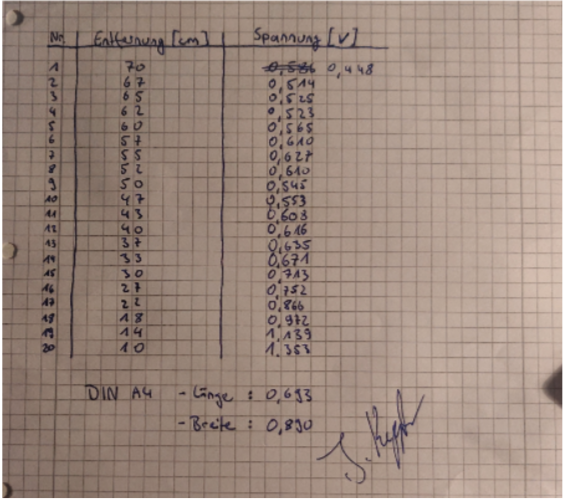
\includegraphics[scale=0.6]{media/messergebnisse.png}
\end{figure}
\end{document}
%------------------------------------
% ╔═╗╔╗╔╔╦╗  ╔╦╗╔═╗╔═╗╦ ╦╔╦╗╔═╗╔╗╔╔╦╗
% ║╣ ║║║ ║║   ║║║ ║║  ║ ║║║║║╣ ║║║ ║ 
% ╚═╝╝╚╝═╩╝  ═╩╝╚═╝╚═╝╚═╝╩ ╩╚═╝╝╚╝ ╩ 
%------------------------------------